\LTR
1. Calculate the exact result of $A \otimes C - B \otimes C$ using Kronecker product properties. \\
P.S. Don't forget to write the dimensionality of each matrix. (20 Pts)

$$A = \begin{bmatrix}
1405 & 1405 & 1405 & 1405 & 1405 \\
0 & 1405 & 1405 & 1405 & 1405 \\
0 & 0 & 1405 & 1405 & 1405 \\
0 & 0 & 0 & 1405 & 1405 \\
0 & 0 & 0 & 0 & 1405
\end{bmatrix}, B = \begin{bmatrix}
1404 & 1405 & 1405 & 1405 & 1405 \\
0 & 1404 & 1405 & 1405 & 1405 \\
0 & 0 & 1404 & 1405 & 1405 \\
0 & 0 & 0 & 1404 & 1405 \\
0 & 0 & 0 & 0 & 1404
\end{bmatrix},$$

$$C = \begin{bmatrix}
2026 & 2026 & 2026 \\
2026 & 2026 & 2026 \\
2026 & 2026 & 2026
\end{bmatrix}$$

2. What does the following Venn Diagram present in terms of Set theory? (15 Pts)

% Note: You will need \usepackage{tikz} in your preamble to render the diagram.
\begin{center}
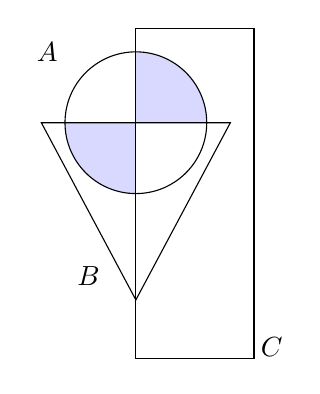
\begin{tikzpicture}[scale=1.5]
    % Define the shapes
    \def\circleA{(0,0) circle (0.6cm)}
    \def\triangleB{(-0.8,0) -- (0.8,0) -- (0,-1.5) -- cycle}
    \def\rectC{(0,-2) rectangle (1,0.8)}

    % Fill shaded regions
    % Top right hatched/shaded (Inside A, Inside C, Outside B)
    \begin{scope}
        \clip \rectC;
        \clip \circleA;
        \fill[blue!15] (0,0) rectangle (0.8,0.8);
    \end{scope}

    % Bottom left hatched/shaded (Inside A, Inside B, left side)
    \begin{scope}
        \clip \triangleB;
        \clip \circleA;
        \fill[blue!15] (-0.8,0) rectangle (0,-0.8);
    \end{scope}

    % Draw outlines
    \draw \circleA;
    \draw \triangleB;
    \draw \rectC;

    % Vertical line splitting the circle and triangle
    \draw (0,0) -- (0,-2);
    % Horizontal line for the top of the rectangle if needed, but it's part of rectC

    % Labels
    \node at (-0.75, 0.6) {$A$};
    \node at (-0.4, -1.3) {$B$};
    \node at (1.15, -1.9) {$C$};
\end{tikzpicture}
\end{center}

\vspace{2em}

3. Suppose lung cancer (A) is either the result of breathing polluted air for a long time (B1), or chemical steams (B2), or smocking cigarette (B3). For a specific person having lung cancer we are interested to know the probability of his/her cancer being the result of polluted air. We know the followings:
\[
P(A|B1) = 0.3, \qquad P(A|B2) = 0.5, \qquad P(A|B3) = 0.4
\]
Suppose the marginal likelihood of B1, B2, B3 partitions are 0.7, 0.05, 0.25, respectively. (25 Pts)

\vspace{2em}

4. We have 12 balls which all have the same weight except for one of them. We are interested in finding the ball which is lighter/heavier using a scale. In the first weighting phase, we decide to pick 8 of these 12 balls randomly and put 4 balls in each pan of our scale. Could you calculate the \underline{\textbf{Expected Information (i.e. The Entropy H)}} that this experiment gives us? Call this H1.

Also calculate the E of the experiment when picking all 12 balls and placing 6 balls in each pan. Let's call this H2.

Compare H1 and H2. Explain your understanding in a couple of sentences. (Hint: You have to calculate the probability of each event, calculate $p \log p$ of each event and sum them up to obtain the expected value. For example, in H2 case, the probability that the first pan is heavier than the second pan is equal to the probability of the revere event which are equal to 0.5). (40 Pts)
\RTL